\chapter{Implementation}
\label{ch:implementation}


In this chapter, details of the implementation practical part of the study is discussed. The architecture, modules, development tools, installation, and configurations of such part are the main role of this chapter.    
\section {Architecture}

	\begin{figure}[ht]
	\begin{center}
		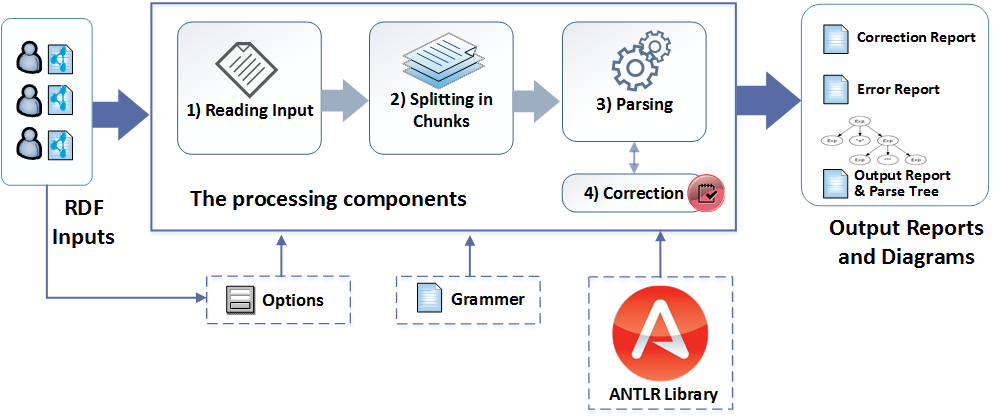
\includegraphics[scale=0.5,angle=0]{images/Architecture}
		\caption{The proposed solution architecture}
		\label{Fig:Architecture}
	\end{center}
\end{figure}
\section {Modules} 
After briefing the proposed solution architecture, It is the time to cover it in more details by shedding light onto those modules which represent the pillars of such solution. The following text discusses 3 main modules of this solution:  
\section{Real-World Use Cases}
In this section, some of use cases tackled in this study to detect syntax errors in RDF input and  the method of error correction of some of those detected syntax error will be exposed. As a start, let's begin with a Turtle example which has no syntax errors, then some syntax errors can be included, then the process of handling them can explained. 
	\vspace{5mm} %5mm vertical space

Listing \ref{lst:turtleExample} shows a Turtle example without syntax errors. First 4 lines are directives or prefixes declaration. 

\begin{lstlisting}[label=lst:turtleExample, numbers=left, caption={RDF example in Turtle serialization format}]
<@\textcolor{blue}{@prefix}@>  <@\textcolor{red}{rdf}@>: <@\textcolor{orange}{<http://www.w3.org/1999/02/22-rdf-syntax-ns#>}@> .
<@\textcolor{blue}{@prefix}@>  <@\textcolor{red}{rdfs}@>:  <@\textcolor{orange}{<http://www.w3.org/2000/01/rdf-schema#>}@> .
<@\textcolor{blue}{@prefix}@>  <@\textcolor{red}{ex}@>:  <@\textcolor{orange}{<http://example.org/>}@> .
<@\textcolor{blue}{@prefix}@>  <@\textcolor{red}{zoo}@>:   <@\textcolor{orange}{<http://example.org/zoo/> }@> .
<@\textcolor{red}{ex}@>:dog1  <@\textcolor{red}{rdf}@>:type  <@\textcolor{red}{ex}@>:animal .
<@\textcolor{red}{ex}@>:cat1  <@\textcolor{red}{rdf}@>:type  <@\textcolor{red}{ex}@>:cat ;
         <@\textcolor{red}{rdfs}@>:label   <@\textcolor{green}{"Lusi"@en}@> .
<@\textcolor{red}{ex}@>:cat  <@\textcolor{red}{rdfs}@>:subClassOf  <@\textcolor{red}{ex}@>:animal .
<@\textcolor{red}{zoo}@>:host  <@\textcolor{red}{rdfs}@>:range  <@\textcolor{red}{ex}@>:animal .
<@\textcolor{red}{ex}@>:zoo1  <@\textcolor{red}{zoo}@>:host  <@\textcolor{red}{ex}@>:cat2 .
\end{lstlisting}










